\documentclass[autodetect-engine,dvipdfmx-if-dvi,ja=standard]{bxjsarticle}

% 二段組にするとき
% \documentclass[twocolumn,autodetect-engine,dvipdfmx-if-dvi,ja=standard]{bxjsarticle}

\usepackage{graphicx}        %図を表示するのに必要
\usepackage{color}           %jpgなどを表示するのに必要
\usepackage{amsmath,amssymb} %数学記号を出すのに必要
\usepackage{setspace}
\usepackage{eclclass}
\usepackage{cases}
\usepackage{here}
\usepackage{fancyhdr}
\usepackage{ascmac}

% 文書全体のスタイルを設定(主に余白)
\setlength{\topmargin}{-0.3in}
\setlength{\oddsidemargin}{0pt}
\setlength{\evensidemargin}{0pt}
\setlength{\textheight}{44\baselineskip}

% 行頭の字下げをしない
\parindent = 0pt

% ヘッダとフッタの設定
\lhead{電気情報工学応用実験II}
\chead{}
\rhead{5E 20番 佐藤凌雅}
\lfoot{}
\cfoot{-\thepage-} % ページ数
\rfoot{}

% 式の番号を(senction_num.num)のようにする
\makeatletter
\@addtoreset{equation}{section}
\def\theequation{\thesection.\arabic{equation}}
\makeatother

% 画像の貼り付けを簡単にする
\newcommand{\pic}[2]
{
  \begin{figure}[H]
    \begin{center}
      \includegraphics[scale=#2]{#1}
    \end{center}
  \end{figure}
}

% 単位の記述を簡単にする
\newcommand{\unit}[1]
{
  \, [\mathrm{#1}]
}
\begin{document}
% \maketitle
\pagestyle{fancy}
\section{目的}
 周波数変調の概念を理解するとともに、その復調を理解する。

\section{理論}
\subsection{FM変調}
 信号を遠距離に伝送するためには変調を行なう必要がある。搬送波の振幅を1m、搬送波の角周波数を$\omega_c(= 2 \pi f_c)$、位相角を$\phi$とすると、信号は式(1) と表わすことができる。
\begin{flalign}
  i &= I_m \sin(\omega_c t + \phi)\nonumber\\
  &= I_m \sin(2 \pi f_c t + \phi)
\end{flalign}

搬送波の振幅$I_n$を変化させると振幅変調、周波数の$\omega_c/2\pi$を変化させると周波数変調、位相角$\phi$を変化させると位相変調になる。

\begin{figure}[H]
  \centering
  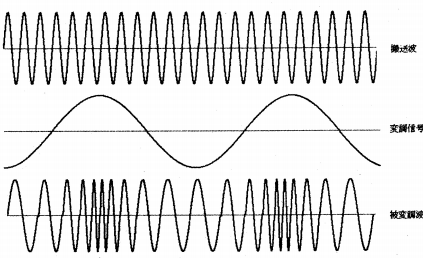
\includegraphics[height=5cm]{./data/1.png}
  \caption{周波数変調波}
\end{figure}

周波数変調(以下、FM と略)の一般式は、信号波の角周波数を$\omega_s$とすると Equation(2) で表わされる。
\begin{flalign}
  i &= I_m \sin(\omega_c t + \frac{\Delta \omega}{\omega_s} \sin\omega_s t)
\end{flalign}

ここで,$\frac{\Delta \omega}{\omega_s} = m_f$で表わすと、

\begin{flalign}
  i &= I_m \sin(\omega_c t + m_f \sin \omega_s t) \nonumber\\
  &= I_m(\sin(\omega_c t) \cos(m_f \sin \omega_s t) + cos\omega_s t \sin(\omega_s t))
\end{flalign}


% 上記 Equation(3) を解くことになるのだが、FM を解くためにはベッセル関数というものを使用する。 ベッセル関数とは、正弦関数または余弦関数の変数が正弦関数であるようなものをいい、その中でも FM では第一種ベッセル関数を使用し、Equation(4)、Equation(5)で表わされる。
% sin(x sine) = 2ji(x) sin + 2js(x) sin 30 + 2js(x) sin 50 + ....... cos(x sin ) = jo(x) + 2jz(x) cos 20 + 2j4(x) cos 40 + ......
% Equation(3) を Equation(4) と Equation(S)に当てはめると Equation(6) となる。
% i = Im{iomf sin wct
% +jims sin(wc + tug) - jims sin(uc-wg). 第1上側帯波と下側帯波 , +jams sin(wc + 2wg) - jams sin(wc - 20g)|第2上側帯波と下側帯波 +jams sin(we + 30g) - jams sin(wc - 30g)第3上側帯波と下側帯波 +jamy sin(ac + 40g) - jamy sin(we - 40g)t ......} 第4上側帯波と下側帯波
% (6)
% 単一周波数で変調しても、Equation(6) のように無数の側帯波が表われる。

\newpage
\subsection{FM復調}
 FM 変調波から元の変調信号を取り出す復調器は、一般に周波数弁別器 (discriminator) が用いら れる。\\
 FM変調波などでの角度変調波の復調には、入力信号の周波数変化と直線的に比例した電圧または 電流を取り出す回路が必要であり、この作用を行なわせる回路が周波数弁別器である。弁別器は、一般にFM波をAM波に変換する回路とAM波を包絡線検波する回路の組み合わせからなる。その特性を図2に示す。\\

\begin{figure}[H]
  \centering
  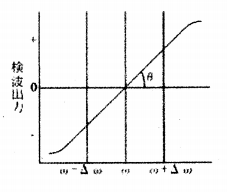
\includegraphics[height=5cm]{./data/2.png}
  \caption{周波数弁別器の特性}
\end{figure}

 FM復調回路の種類としては、スロープ検波回路、離調形弁別回路、フォスター・シーレ回路、比検波回路、C結合形回路、乗算形回路などがある。\\

\subsubsection{フォスター・シーレ回路}
 周波数の変化を振幅の変化した信号に変換した後 AM復調することで検波を行う.\\
 真空管時代から存在する古典的な回路.\\
 ダイオードに特性の揃ったものが必要なことと、良い特性を出すには回路設計と調整が難しい。\\
 入力信号の周波数が高くなると出力電圧が正に増加、周波数が低くなると負に増加する特性を持つ.\\

\section{実験回路図}
\subsection{周波数変調回路}
\begin{figure}[H]
  \centering
  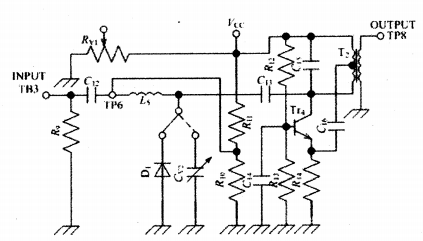
\includegraphics[height=5cm]{./data/3.png}
  \caption{周波数変調回路}
\end{figure}

\subsection{周波数復調回路}
\begin{figure}[H]
  \centering
  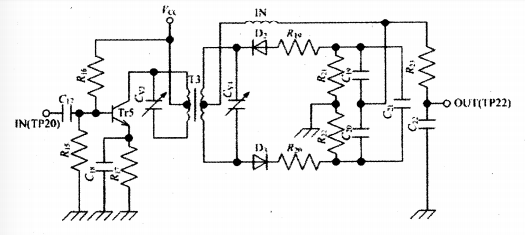
\includegraphics[height=5cm]{./data/4.png}
  \caption{周波数復調回路}
\end{figure}

\section{使用機器}
周波数変調復調実験装置\\
オシロスコープ\\
直流電源\\
テスタ\\
ファンクションジェネレータ\\
スペクトラムアナライザ\\
周波数カウンター\\
低周波発振器\\

\section{実験方法}
\subsection{周波数変調実験}
\subsubsection{直流入力周波数特性}
\begin{enumerate}
  \item 直流入力用ボリューム RV1 の中間端子 TP3と変調回路TP6を接続し、TP6の電圧を測定できるようにテスタを接続する。\\
  \item 出力端子 TP8に周波数カウンターを接続する。\\
  \item 切替スイッチ SW3を可変容量ダイオード(バリキャップ)$D_1$側に切替え、電源スイッチを投入する。\\
  \item RV1を調整して入力電圧を0から2Vごとに12Vまで変化させ周波数の変化を測定しグラフにまとめる。\\
\end{enumerate}

\subsubsection{交流入力周波数特性}
\begin{enumerate}
  \item 入力端子TB3にファンクションジェネレータを接続する。\\
  \item TP4とTP8にオシロスコープを接続する。\\
  \item 発振器から1Hzの正弦波を出力する。\\
  \item 入力電圧の振幅で出力周波数が変化することを確認し、波形を連続写真撮影する。\\
  \item TP8にスペクトラムアナライザを接続し任意の周波数を入力した場合の変調波スペクトラムを確認・測定する。\\
\end{enumerate}

\section{周波数復調実験}
\begin{enumerate}
  \item 入力端子 TP20 にファンクションジェネレータ、出力端子TP22にテスタ (電圧計)を接続する。\\
  \item ファンクションジェネレータからFM受信機の中間周波数10.70MHz、0.7$V_{p-p}$を入力し、出力がOV付近になるように可変コンデンサ$C_V4$を調整する。\\
  \item 周波数を「中間周波数 +200kHz」に変化させて、出力が最大値を得られるように$C_V3$を調整する。\\
  \item 周波数を「中間周波数 -200kHz」に変化させて、出力が最小値を得られるように$C_V3$を調整する。\\
  \item 周波数を中間周波数に戻し出力が最初に調整した電圧付近 (0V 付近)であることを確認する。\\
  \item 入力周波数に対する出力電圧を測定する。入力周波数の変化は 0.05MHz ごとに変化させ、±方向の電圧がピークを超えるまで測定すること。
\end{enumerate}

\end{document}
